%
% flocker_ui.tex
% @author Sidharth Mishra
% @description 
% @copyright  BSD 3-Clause License
%
% Copyright (c) 2018, Sidharth Mishra
% All rights reserved.
%
% Redistribution and use in source and binary forms, with or without
% modification, are permitted provided that the following conditions are met:
%
% * Redistributions of source code must retain the above copyright notice, this
%  list of conditions and the following disclaimer.
%
% * Redistributions in binary form must reproduce the above copyright notice,
%  this list of conditions and the following disclaimer in the documentation
%  and/or other materials provided with the distribution.
%
% * Neither the name of the copyright holder nor the names of its
%  contributors may be used to endorse or promote products derived from
%  this software without specific prior written permission.
%
% THIS SOFTWARE IS PROVIDED BY THE COPYRIGHT HOLDERS AND CONTRIBUTORS "AS IS"
% AND ANY EXPRESS OR IMPLIED WARRANTIES, INCLUDING, BUT NOT LIMITED TO, THE
% IMPLIED WARRANTIES OF MERCHANTABILITY AND FITNESS FOR A PARTICULAR PURPOSE ARE
% DISCLAIMED. IN NO EVENT SHALL THE COPYRIGHT HOLDER OR CONTRIBUTORS BE LIABLE
% FOR ANY DIRECT, INDIRECT, INCIDENTAL, SPECIAL, EXEMPLARY, OR CONSEQUENTIAL
% DAMAGES (INCLUDING, BUT NOT LIMITED TO, PROCUREMENT OF SUBSTITUTE GOODS OR
% SERVICES; LOSS OF USE, DATA, OR PROFITS; OR BUSINESS INTERRUPTION) HOWEVER
% CAUSED AND ON ANY THEORY OF LIABILITY, WHETHER IN CONTRACT, STRICT LIABILITY,
% OR TORT (INCLUDING NEGLIGENCE OR OTHERWISE) ARISING IN ANY WAY OUT OF THE USE
% OF THIS SOFTWARE, EVEN IF ADVISED OF THE POSSIBILITY OF SUCH DAMAGE.
%
% @created Sat Mar 31 2018 22:06:06 GMT-0700 (PDT)
% @last-modified Wed Apr 04 2018 22:21:51 GMT-0700 (PDT)
%


\documentclass[../main]{subfiles}

\begin{document}

\section{Flocker UI}
\label{flockerUI}

{\em Flocker UI} is divided into two separate areas: the {\em canvas area}, and the {\em sidebar area}. Width and height of the {\em canvas area} and {\em sidebar area} are auto-configurable -- they adjust according the size of the browser window. Features and styles of the UI component have been implemented using {\em jQuery2.1} \cite{jquery} and {\em CSS3} \cite{css3}.

{\em Note}: We recommend viewing the simulation on a screen with resolution of \code{1920 x 1080} or \code{FHD} in {\em full-screen} mode for best experience.

\subsection{Canvas Area}
\label{canvasArea}

The {\em canvas area} -- or {\em content area} -- holds the simulation. The user can add new swallows to the simulation by clicking on the {\em canvas area}. When the mouse is over the {\em canvas area}, the cursor changes into a {\em swallow}~[Fig. \ref{swallowImg}]. We designed this as an affordance to notify the user that they are on a region where swallows can be added. The cursor is the image of a swallow of dimensions \code{100 x 100 pixels}. The canvas is generated by the {\em flocker core} covered in [Section \ref{flocker}].

Although the canvas is {\em white} (\code{\#ffffff}) in color by default, we allow the user to change the background color of the canvas by using the \code{R}, \code{G}, and \code{B} (Red, Green, and Blue) sliders [Fig. \ref{colorSliders}] available on the {\em sidebar}. The \code{R}, \code{G}, and \code{B} values can be controlled by using the range sliders or input boxes on the {\em sidebar}. If the range slider is dragged in the positive x-direction or negative x-direction, it will increase or decrease the intensity of the respective color.

\begin{figure}
	\centering
	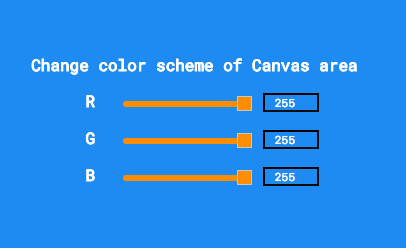
\includegraphics[scale=0.35, width=250pt, frame]{resources/color_sliders.png}
	\caption{The color sliders and input boxes.}
	\label{colorSliders}
\end{figure}

Alternatively, the user could also use the corresponding input box to enter the exact value for the desired color. Since the input box and sliders are normal {\em HTML DOM elements}, they can be cycled through -- selected -- using the \code{TAB} button as usual. The user also gets the ability to increase or decrease the value entered in the input boxes by holding the {\em up arrow key} or {\em down arrow key}. Using the mouse scroll wheel also results in the same effect. Furthermore, when the input box is in focus, it gains an affordance on the right edge [Fig. \ref{forceSliders}]  enabling the user to increment/decrement the value entered. If the user specifies the intensity of the color above \code{255} or below \code{0} in the input box, they get an error and are asked to specify the value within the range~\code{0-255}.

\subsection{Sidebar Area}
\label{sidebarArea}

The {\em sidebar} holds the controllers for the simulation. It is located on the left of the webpage. It is separated from the {\em canvas/content area} by a {\em split-bar}. The width of the {\em sidebar area} is changed by dragging the {\em split-bar} horizontally to the right or left. The {\em sidebar} is {\em flexible} and gains a {\em scrollbar} when it doesn't find the browser-window's width to be sufficient for rendering itself. We change the mouse pointer to the \mbox{\em col-resize} pointer to let the user know that they are on the {\em split-bar}. This afforance notifies the user that they can drag to resize the {\em sidebar area}. The sidebar is restricted to be resized between the range \code{300-400~pixels} to prevent the UI from distorting.

To control the {\em cohesion}, {\em alignment}, and {\em separation} steering forces of the simulation, range sliders and input boxes are provided [Fig. \ref{forceSliders}]. We limit the weights of these forces to the range \code{0-5 units} and allow changes in steps of \code{0.1 units}. Similarly, we limit the desired strength of these forces to the range \code{0-300 units} and allow changes in steps of \code{5 units}. The controllers used for force manipulation have the same operation mechanism as the ones used for manipulating canvas's background color intensities.

Initially, we had two groups of controllers. The first group had controllers for manipulating the strength of all the forces, and the second group had controllers for manipulating the weights of all the forces. However, we found this layout for controllers lacked coherence and moved over to our current layout. We have grouped the {\em desired strength} and {\em desired weight} controllers of the same force together to provide better coherence.

\begin{figure}
	\centering
	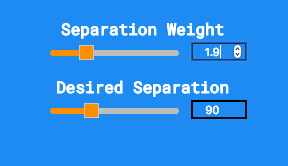
\includegraphics[scale=0.35, width=250pt, frame]{resources/force_sliders.png}
	\caption{The force strength and weight controllers.}
	\label{forceSliders}
\end{figure}

The controllers consist of a range slider and an input box. The range slider and contents of the input box are {\em in-sync} with each other -- when one changes, the other reflects the change. When bad values are entered in the input boxes, an error message is displayed below the controller specifying the valid range of values. One would argue, it is better to notify the user about the range of values upfront but, we have chosen not to. We believe that the user will not be entering bad values most of the time. Rather than crowding the space with extra information, we chose to gently warn the user when they made the mistake of entering bad values into the input boxes. This results in a cleaner UI that is not cramped -- less noise allows for a better simulation experience.

\subsection{Color scheme}
\label{colorScheme}

We followed the theory of {\em complementary colors} as mentioned in \cite{colorTheory}. We decided to make the sidebar {\em blue} (\code{\#2196f3}). Following the theory of complementary colors, we chose the color of the sliders to be {\em orange} (\code{\#ff9800}). This makes them {\em pop-out} over the background. We chose the color of the text to be {\em white} (\code{\#ffffff}) and the color of the borders of input boxes to be {\em black} (\code{\#000000}). The canvas was left {\em white} by default but, the user gets the controllers to change the canvas' background color.

\subsection{Testing the UI}
\label{uiTesting}

We tested the UI on various screen sizes and browser-window sizes. The viewing experience is the best on screens with atleast \code{1920 x 1080} or \code{FHD} resolution. We have implemented the {\em sidebar} and {\em canvas} to be flexible -- using CSS3 {\em flexbox} -- so, they adjust to the screen space available automatically. We tested the {\em frame-rate and swallow count} text alignment for various screen sizes by using the debug grid. It worked fine for most screen/browser window sizes. The controls were tested by entering valid and invalid values into the input boxes. The synchronization between the slider control and the input box contents was also tested by changing the values. The slider and input box contents are in-sync and bad values display the desired error messages.

\end{document}